
%\documentclass[12pt,draft]{article}
\documentclass[12pt]{article}


\usepackage[english]{babel}
%\usepackage[frenchb]{babel}
\usepackage{CJK}
\usepackage{mathrsfs}
\usepackage{amsmath,amsthm,amsfonts,amssymb}
\usepackage{geometry}
\usepackage{fancyhdr}
\usepackage{indentfirst}
\usepackage{float}
\usepackage[dvips]{graphicx}
\usepackage{subfigure}
\usepackage[font=small]{caption}
\usepackage{threeparttable}
\usepackage{cases}
\usepackage{multicol}
\usepackage{url}
\usepackage{amsmath}
\usepackage{bm}
\usepackage{xcolor}
\usepackage{overpic}
\usepackage{natbib}
\usepackage[utf8]{inputenc}

\usepackage{natbib}
\usepackage{graphicx}
\usepackage{hyperref}
\numberwithin{equation}{section}


\geometry{left=1.5cm,right=1.5cm,top=1.5cm,bottom=1.5cm}
\setlength{\parskip}{0.3\baselineskip}
\setlength{\headheight}{15pt}
\begin{document}\small
  \renewcommand\figurename{Fig.}
  %\renewcommand\arraystretch{1.0}
    \title{Probalistic Graphic Model\cite{Coursera}\cite{koller2009probabilistic} Notes}
    \author{Yan JIN}
    \pagestyle{fancy}\fancyhf{}
    \lhead{}\rhead{JIN Yan}
    \lfoot{\textit{}}\cfoot{}\rfoot{\thepage}
    \renewcommand{\headrulewidth}{1.pt}
    \renewcommand{\footrulewidth}{1.pt}
  \maketitle
  
\tableofcontents
\newpage

\section{Introduction and Overview}
Model: The model is a \textbf{declarative representation} of our understanding of the world. It's \textbf{declarative} means that the representation stands on its own, which means that we can look into it and make sense of it \textbf{aside from any algorithm} that we might choose to apply on. 


\begin{enumerate}
	\item Representation
	
	- Directed and undirected
	
	- Temperal and plate models
	\item Inference
	
	- Exact and approximate
	
	- Decision making
	\item Learning
	
	- Parameters and structure
	
	- With and without complete data
\end{enumerate}

\subsection{Distributions}
Chapters 2.1.1 to 2.1.3.
\subsection{Factors}
Chapter 4.2.1.
\subsection{Quiz}
\begin{figure}[H]
  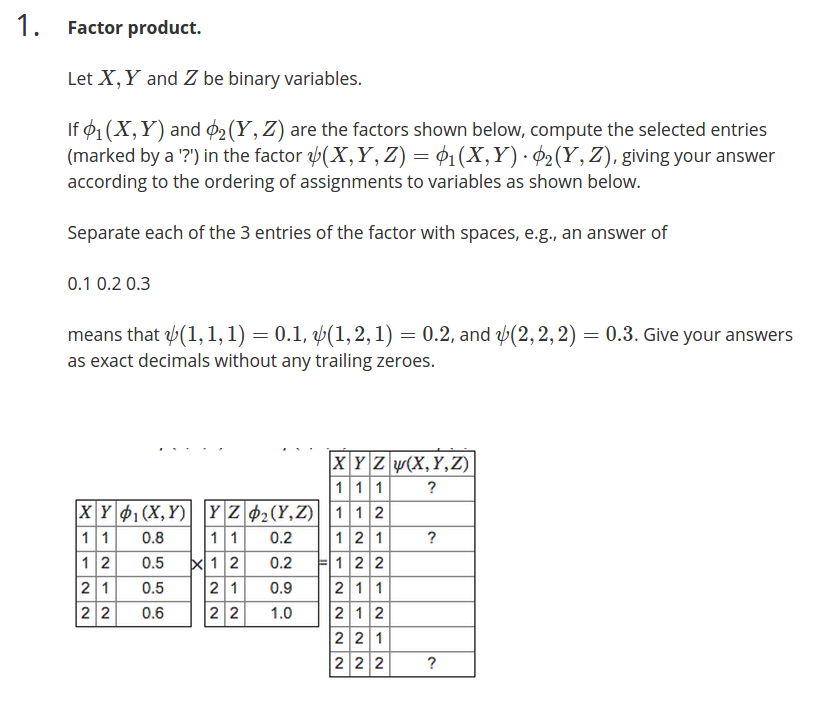
\includegraphics[width=\linewidth]{PGMpics/01-01.png}
  \caption{Exercise 01-01}
  \label{fig:Exercise01-01}
\end{figure}

\begin{figure}[H]
  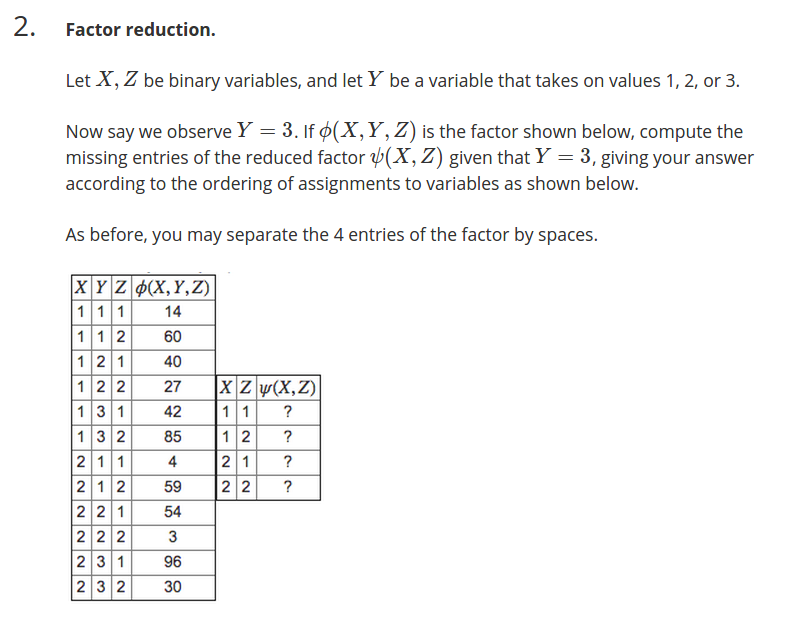
\includegraphics[width=\linewidth]{PGMpics/01-02.png}
  \caption{Exercise 01-02}
  \label{fig:Exercise01-02}
\end{figure}

\begin{figure}[H]
  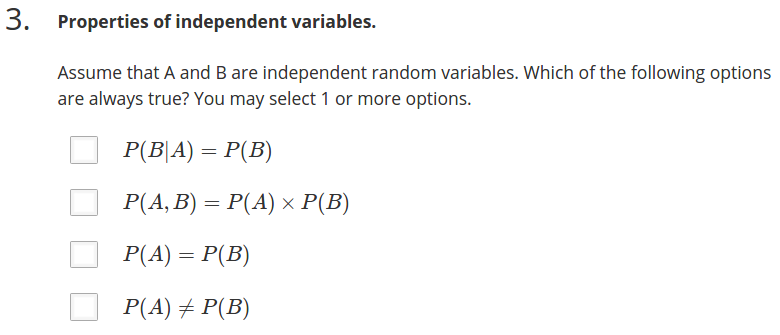
\includegraphics[width=\linewidth]{PGMpics/01-03.png}
  \caption{Exercise 01-03}
  \label{fig:Exercise01-03}
\end{figure}

\begin{figure}[H]
  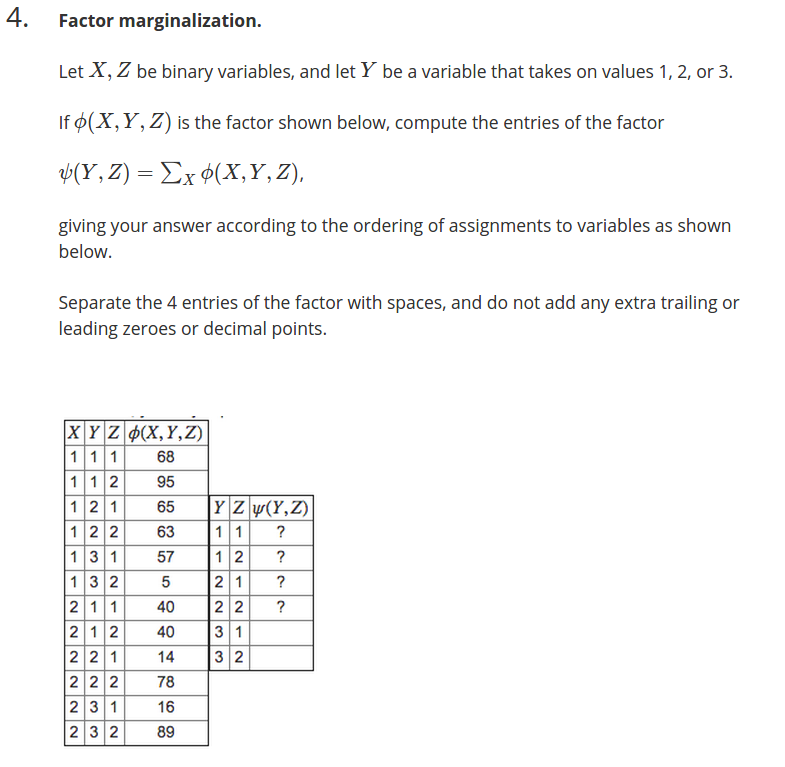
\includegraphics[width=\linewidth]{PGMpics/01-04.png}
  \caption{Exercise 01-04}
  \label{fig:Exercise01-04}
\end{figure}

My answers for the Quiz:

01-01: 0.16 0.45 0.6

01-02: 42 85 96 30

01-03: choose 1 and 2

01-04: 190 163 70 207

\section{Representation}
\subsection{Baysian Network (Directed Models)}
\subsubsection{Baysian Network Fundamentals}
\subsubsection{Semantics and Factorization}
Chapters 3.2.1, 3.2.2. If you are unfamiliar with genetic inheritance, please watch this short \href{https://www.khanacademy.org/science/biology/classical-genetics/mendelian--genetics/v/introduction-to-heredity}{Khan Academy video} for some background.
\subsubsection{Reasoning Patterns}
Chapter 3.2.1.
\subsubsection{Flow of Probabilistic Influence}
Chapter 3.3.1.
\subsubsection{Bayesian Networks: Independencies}

Conditional Independence. Chapters 2.1.4, 3.1.

Independencies in Bayesian Networks. Chapter 3.2.2.

Naive Bayes. Chapter 3.1.3.

Bayesian Networks: Knowledge Engineering

Application - Medical Diagnosis Chapter 3.2: Box 3.D (p. 67).

\subsection{Template Models for Bayesian Networks}

Overview. Chapter 6.1.

Temporal Models - DBNs. Chapters 6.2, 6.3.

Temporal Models - HMMs. Chapters 6.2, 6.3.

Plate Models. Chapter 6.4.1.

\subsection{Structured CPDs for Bayesian Networks}

Overview. Chapters 5.1, 5.2.

Tree-Structured CPDs. Chapter 5.3.

Independence of Causal Influence. Chapter 5.4.

Continuous Variables. Chapter 5.5.

\subsection{Markov Network Fundamentals (Undirected Models)}

Pairwise Markov Networks. Chapter 4.1.

General Gibbs Distribution. Chapter 4.2.2.

Conditional Random Fields. Chapter 4.6.1.

Independencies in Markov Networks and Bayesian Networks

Independencies in Markov Networks. Chapter 4.3.1.

I-Maps and Perfect Maps. Chapter 3.3.4.

Local Structure in Markov Networks

Log-Linear Models. Chapter 4.4, p. 125.

Shared Features in Log-Linear Models. Chapter 4: Box 4.B (p. 112), Box 4.C (p. 126), Box 4.D (p. 127).

\subsection{Decision Making}

Maximum Expected Utility Chapter 22.1.1, 23.2.104, 23.4.1-2, 23.5.1

Utility Functions Chapter 22.2.1-3, 22.3.2, 22.4.2

Value of Perfect Information Chapter 23.7.1-2

\subsection{Knowledge Engineering \& Summary}

\renewcommand\refname{Reference}
\bibliographystyle{plain}
\bibliography{PGM}

  \clearpage
\end{document}